\section{Random, but useful stuff}

\sep
\subsection{Trigonometrie}

\[\sin z = z - \frac{z^3}{3!} + \frac{z^5}{5!} - \frac{z^7}{7!} + \cdots = \sum_{n=0}^\infty \frac{(-1)^n z^{2n + 1}}{(2n + 1)!} \]

\[\cos z = 1 - \frac{z^2}{2!} + \frac{z^4}{4!} - \frac{z^6}{6!} + \cdots = \sum_{n=0}^\infty \frac{(-1)^n z^{2n}}{(2n)!} \]

\[ \exp(z) = 1 + z + \frac{z^2}{2!} + \frac{z^3}{3!}  + \frac{z^4}{4!} + \cdots = \sum_{n=0}^\infty \frac{x^n}{n!} \]

\[ \log(x + 1) = \sum_{n=1}^\infty \frac{(-1)^{n - 1}}{n} x^n \quad \text{ für } -1 < x < 1\]
\Satz[3.8.1] $\sin, \  \cos \text{ und } \exp$ sind stetig auf $\R$

\sep

\subsubsection{Additionstheoreme} 

\begin{flalign}
& \sin \Big(\frac{\pi}{2} - \alpha \Big) = \cos \alpha  & \nonumber \\
& \cos \Big( \frac{\pi}{2} + \alpha \Big) = \sin(\alpha) & \nonumber \\
& \tan \Big( \frac{\pi}{2} - \alpha \Big) = \frac{1}{\tan \alpha }& \nonumber \\
& \sin( - \alpha) = - \sin \alpha & \nonumber  \\
& \cos( - \alpha) = \cos \alpha & \nonumber  \\
& \tan(- \alpha) = - \tan \alpha & \nonumber \\
& \sin ( \alpha \pm \beta ) = \sin \alpha \cos \beta \pm \cos \alpha \sin \beta & \nonumber \\ 
& \cos( \alpha \pm \beta ) = \cos \alpha \cos \beta \mp \sin \alpha \sin \beta & \nonumber \\
& \tan( \alpha \pm \beta) = \frac{\tan \alpha \pm \tan \beta}{1 \mp \tan \alpha \tan \beta} & \nonumber \\
& \sin ( 2 \alpha) = 2 \sin \cos \alpha & \nonumber \\
& \cos( 2 \alpha) = \cos^2 \alpha - \sin^2 \alpha = 2 \cos^2 \alpha - 1 & \nonumber \\
& \tan( 2 \alpha) = \frac{2 \tan \alpha}{4 - \tan^2 \alpha} & \nonumber \\
& \sin( 3 \alpha) = 3 \sin \alpha - 4 \sin^3 \alpha & \nonumber \\
& \cos(3 \alpha) = 4 \cos^3 \alpha - \cos \alpha & \nonumber \\
& \tan(3 \alpha) = \frac{3 \tan \alpha - \tan^3 \alpha}{1 - 3 \tan^2 \alpha} & \nonumber \\
& \sin^2 \Big(\frac{\alpha}{2} \Big) = \frac{1 - \cos \alpha}{2} & \nonumber \\
& \cos^2 \Big(\frac{\alpha}{2} \Big) = \frac{1 + \cos \alpha}{2} & \nonumber  \\
& \tan^2 \Big(\frac{\alpha}{2} \Big) = \frac{1 - \cos \alpha}{1 + \cos \alpha} & \nonumber \\
& \tan \Big(\frac{\alpha}{2} \Big) = \frac{1 - \cos \alpha}{\sin \alpha} = \frac{\sin \alpha}{1 + \cos \alpha} & \nonumber \\
& \sin \alpha + \sin \beta = 2 \sin \frac{\alpha + \beta}{2} \cos \frac{\alpha - \beta}{2} & \nonumber \\
& \sin \alpha - \sin \beta = 2 \cos \frac{\alpha + \beta}{2} \sin \frac{\alpha - \beta}{2} & \nonumber \\
& \cos \alpha + \cos \beta = 2 \cos \frac{\alpha + \beta}{2} \cos \frac{\alpha - \beta}{2} & \nonumber \\
& \cos \alpha - \cos \beta = - 2 \sin \frac{\alpha + \beta}{2} \sin \frac{\alpha - \beta}{2} & \nonumber \\
& \sin \alpha \sin \beta = \frac{1}{2} [ \cos ( \alpha - \beta) - \cos (\alpha + \beta)] & \nonumber \\
& \cos \alpha \cos \beta = \frac{1}{2} [ \cos ( \alpha - \beta) + \cos( \alpha + \beta)] & \nonumber \\
& \sin \alpha \cos \beta = \frac{1}{2} [ \sin( \alpha - \beta) + \sin( \alpha + \beta) ] & \nonumber \\
& \sin( \arccos(x)) = \sqrt{1 - x^2}  & \nonumber \\
& \cos( \arcsin(x)) = \sqrt{1 - x ^2} & \nonumber
\end{flalign}

\subsubsection{Unit Circle $(\cos(x), \sin(x))$}
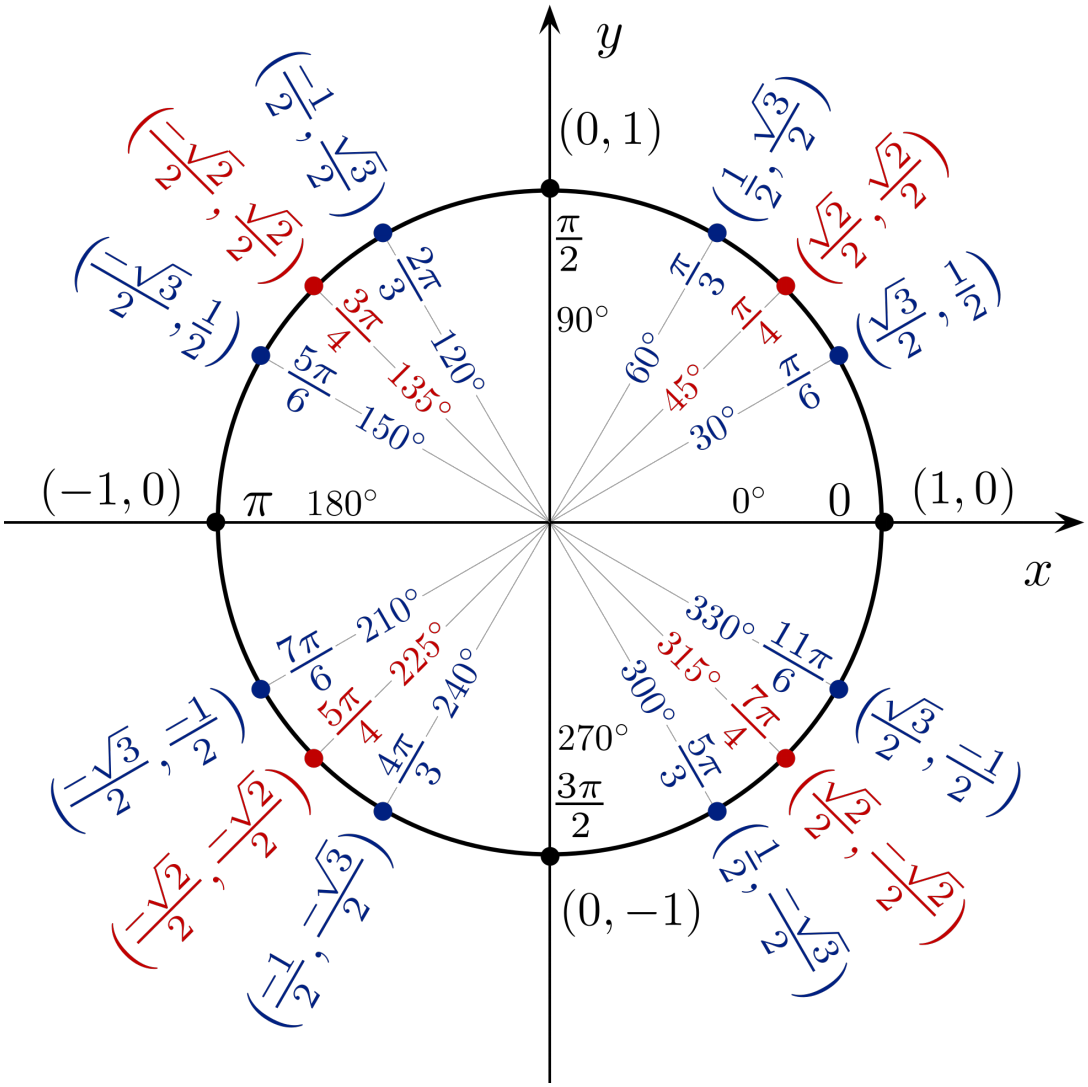
\includegraphics[scale=0.225]{sinus_cosinus}

\sep

\Satz[3.8.2] Eigenschaften von sin und cos
\begin{enumerate}
	\item $\cos z = \cos(-z) \text{ und } \sin(-z) = -\sin(z)$
	\item $\exp(i \cdot z) = \cos(z) + i \cdot \sin(z)$
	\item $\cos(z)^2 + \sin(z)^2 = 1$
	\item $\sin(z+w) = \sin(z) \cdot \cos(w) + \sin(w) \cdot \cos(z)$ \\
	 $\cos(z+w) = \cos(z) \cdot \cos(w) - \sin(w) \cdot \sin(z)$ 
	\item $\sin(z) = \frac{e^{iz}-e^{-iz}}{2i}$, $\cos(z) = \frac{e^{iz}+e^{-iz}}{2}$
\end{enumerate}

\Korollar[3.8.3] \\
\( \sin(2 \cdot z) = 2 \sin(z) \cdot \cos(z) \) \\ 
\(\cos(2 \cdot z) = \cos(z)^2- \sin(z)^2 \)

\sep

\[\sin(t) = t - \frac{t^3}{6} \cos \theta \quad \text{für ein } \theta \in [0,t] \]

\[\sin(x) \leq x \quad \forall  x \geq 0 \]

\[\abs{\sin(x)} \leq \abs{x} \]
\sep

\subsection{Formula for $a x^2 + b x + c = 0$}

\[ x = \frac{-b + \pm \sqrt{b^2 - 4 a c} }{2 a} \]

\sep

\subsection{Konvergente Folgen}
\begin{enumerate}
\item Weierstrass (monoton + beschränkt)
\item Vergleichssatz
\end{enumerate}

\sep

\subsection{Konvergente Reihen}

\begin{enumerate}
\item Weierstrass (monoton + beschränkt)
\item Vergleichssatz
\item Geometrische Folge
\item Alternierende Reihe
\item Riemann Zeta
\item Teleskopieren
\item $\lim \limits_{n \rightarrow \infty} a_n = 0$
\item konvergiert das Integral?
\end{enumerate}

\sep

\subsection{Implications}

\( \text{f differenzierbar} \implies \text{f stetig} \implies \text{f integrierbar} \)

\sep

\subsection{Länge von Kurven}

\[ L = \int_a^b = \sqrt{x'(t)^2 + y'(t)^2} dt  \quad p(t) = (x(t), y(t))\]

\[ L = \int_c^d = \sqrt{1 + f'(x)^2} dx \quad y = f(x), \ x \in [c, d] \]

